\documentclass[14pt,a4paper]{report}  %紙張設定
\usepackage{xeCJK}%中文字體模組
\setCJKmainfont{標楷體} %設定中文字體
%\setCJKmainfont{MoeStandardKai.ttf}
\newfontfamily\sectionef{Times New Roman}%設定英文字體
%\newfontfamily\sectionef{Nimbus Roman}
\usepackage{enumerate}
\usepackage{amsmath,amssymb}%數學公式、符號
\usepackage{amsfonts} %數學簍空的英文字
\usepackage{graphicx, subfigure}%圖形
\usepackage{fontawesome5} %引用icon
\usepackage{type1cm} %調整字體絕對大小
\usepackage{textpos} %設定文字絕對位置
\usepackage[top=2.5truecm,bottom=2.5truecm,
left=3truecm,right=2.5truecm]{geometry}
\usepackage{titlesec} %目錄標題設定模組
\usepackage{titletoc} %目錄內容設定模組
\usepackage{textcomp} %表格設定模組
\usepackage{multirow} %合併行
%\usepackage{multicol} %合併欄
\usepackage{CJK} %中文模組
\usepackage{CJKnumb} %中文數字模組
\usepackage{wallpaper} %浮水印
\usepackage{listings} %引用程式碼
\usepackage{hyperref} %引用url連結
\usepackage{setspace}
\usepackage{lscape}%設定橫式
\lstset{language=Python, %設定語言
		basicstyle=\fontsize{10pt}{2pt}\selectfont, %設定程式內文字體大小
		frame=lines,	%設定程式框架為線
}
%\usepackage{subcaption}%副圖標
\graphicspath{{./../images/}} %圖片預設讀取路徑
\usepackage{indentfirst} %設定開頭縮排模組
\renewcommand{\figurename}{\Large 圖.} %更改圖片標題名稱
\renewcommand{\tablename}{\Large 表.}
\renewcommand{\lstlistingname}{\Large 程式.} %設定程式標示名稱
\hoffset=-5mm %調整左右邊界
\voffset=-8mm %調整上下邊界
\setlength{\parindent}{3em}%設定首行行距縮排
\usepackage{appendix} %附錄
\usepackage{diagbox}%引用表格
\usepackage{multirow}%表格置中
%\usepackage{number line}
%=------------------更改標題內容----------------------=%
\titleformat{\chapter}[hang]{\center\sectionef\fontsize{20pt}{1pt}\bfseries}{\LARGE 第\CJKnumber{\thechapter}章}{1em}{}[]
\titleformat{\section}[hang]{\sectionef\fontsize{18pt}{2.5pt}\bfseries}{{\thesection}}{0.5em}{}[]
\titleformat{\subsection}[hang]{\sectionef\fontsize{18pt}{2.5pt}\bfseries}{{\thesubsection}}{1em}{}[]
%=------------------更改目錄內容-----------------------=%
\titlecontents{chapter}[11mm]{}{\sectionef\fontsize{18pt}{2.5pt}\bfseries\makebox[3.5em][l]
{第\CJKnumber{\thecontentslabel}章}}{}{\titlerule*[0.7pc]{.}\contentspage}
\titlecontents{section}[18mm]{}{\sectionef\LARGE\makebox[1.5em][l]
{\thecontentslabel}}{}{\titlerule*[0.7pc]{.}\contentspage}
\titlecontents{subsection}[4em]{}{\sectionef\Large\makebox[2.5em][l]{{\thecontentslabel}}}{}{\titlerule*[0.7pc]{.}\contentspage}
%=----------------------章節間距----------------------=%
\titlespacing*{\chapter} {0pt}{0pt}{18pt}
\titlespacing*{\section} {0pt}{12pt}{6pt}
\titlespacing*{\subsection} {0pt}{6pt}{6pt}
%=----------------------標題-------------------------=%             
\begin{document} %文件
\sectionef %設定英文字體啟用
\vspace{12em}
\begin{titlepage}%開頭
\begin{center}   %標題  
\makebox[1.5\width][s] %[s] 代表 Stretch the interword space in text across the entire width
{\fontsize{24pt}{2.5pt}國立虎尾科技大學}\\[18pt]
\makebox[1.5\width][s]
{\fontsize{24pt}{2.5pt}機械設計工程系}\\[18pt]
\sectionef\fontsize{24pt}{1em}\selectfont\textbf
{
\vspace{0.5em}
cd2023 2a-pj1ag6分組報告}\\[18pt]
%設定文字盒子 [方框寬度的1.5倍寬][對其方式為文字平均分分布於方框中]\\距離下方18pt
\vspace{1em} %下移
\fontsize{30pt}{1pt}\selectfont\textbf{網際手足球場景設計}\\
\vspace{1em}
\sectionef\fontsize{30pt}{1em}\selectfont\textbf
{
\vspace{0.5em}
Web-based Foosball Scene Design}
 \vspace{2em}
%=---------------------參與人員-----------------------=%             
\end{center}
\begin{flushleft}
\begin{LARGE}

\hspace{32mm}\makebox[5cm][s]
{指導教授:\quad 嚴\quad 家\quad 銘\quad 老\quad 師}\\[6pt]
\hspace{32mm}\makebox[5cm][s]
{班\qquad 級:\quad 四\quad 設\quad 二\quad 甲}\\[6pt]
\hspace{32mm}\makebox[5cm][s]
{學\qquad 生:\quad 呂\quad 佳\quad 柔\quad(41023104)}
\\[6pt]
\hspace{32mm}\makebox[5cm][s]
{\hspace{36.5mm}王\quad 啟\quad 騰\quad(41023112)}\\[6pt]
\hspace{32mm}\makebox[5cm][s]
{\hspace{36.5mm}\quad \quad \quad}\\[6pt]
\hspace{32mm}\makebox[5cm][s]
{\hspace{36.5mm}\quad \quad \quad}\\[6pt]
\hspace{32mm}\makebox[5cm][s]
{\hspace{36.5mm}\quad \quad \quad}\\[6pt]
%設定文字盒子[寬度為5cm][對其方式為文字平均分分布於方框中]空白距離{36.5mm}\空白1em
\end{LARGE}
\end{flushleft}
\vspace{6em}
\fontsize{18pt}{2pt}\selectfont\centerline{\makebox[\width][s]
{中華民國\hspace{3em} 
112 \quad 年\quad 3\quad 月}}
\end{titlepage}
\newpage
%=---------------報告製作核可證明---------------------=%
 {\renewcommand\baselinestretch{1.4}\selectfont %設定以下行距
 {\begin{center}
    {\fontsize{20pt}{2.5pt} {國立虎尾科技大學 \qquad 機械設計工程系}\\[8pt]{分組報告製作合格認可證明}\\
    \hspace*{\fill} \\ %似enter鍵換行
    \par}
     \end{center}}
    {\begin{textblock}{60}(1.85,0.8)
    \noindent \fontsize{15pt}{16pt}\selectfont 分組報告製作修習學生\enspace:\quad
    {\begin{minipage}[t]{10em}\underline{四設二甲\enspace 41023104 呂佳柔}\\ \underline{四設二甲\enspace 41023112\enspace 王啟騰}\\ \underline\\ %下劃線符號指令
    \end{minipage}}
         \par} %結束指定行距
    {\renewcommand\baselinestretch{1.2}\selectfont %設定以下行距
    {\begin{textblock}{30}(1.8,4)
    \noindent \fontsize{16pt}{16pt}\selectfont 分組報告題目\enspace :網際手足球場景設計
    \hspace*{\fill} \\
    \hspace*{\fill} \\
    \noindent \fontsize{16pt}{16pt}\selectfont 經評量合格,特此證明
    \hspace*{\fill} \\
    \hspace*{\fill} \\
    \noindent \fontsize{16pt}{16pt} \makebox[6em][s]{評審委員}\enspace:\quad
    {\begin{minipage}[t]{6em} \underline{            }\\[16pt] \underline{            }\\[16pt] \underline{            }\\
    \end{minipage}}
    \end{textblock}}
    {\begin{textblock}{10}(1.8,9)
    {\begin{flushleft}
    \fontsize{16pt}{16pt}\selectfont \makebox[6em][s]{指導老師}\enspace:\quad \underline{            }\\[10pt]
    \hspace*{\fill} \\
    \fontsize{16pt}{2.5pt}\selectfont \makebox[12em][s]{中華民國一一二年}\hspace{2pt}
    \fontsize{16pt}{2.5pt}\selectfont\makebox[8em][s]{四月十七日}
    \end{flushleft}}
    \end{textblock}}
    \end{textblock}}
     \par} %結束指定行距
     \newpage

%=------------------------摘要-----------------------=%
\renewcommand{\baselinestretch}{1.5} %設定行距
\pagenumbering{roman} %設定頁數為羅馬數字
\clearpage  %設定頁數開始編譯
\sectionef
\addcontentsline{toc}{chapter}{摘~~~要} %將摘要加入目錄
\begin{center}
\LARGE\textbf{摘~~要}\\
\end{center}
\begin{flushleft}
\fontsize{14pt}{20pt}\sectionef\hspace{12pt}\quad 本學期採取個人及團體分組來學習,團體實習目標為開發一款能在 web-based CoppeliaSim 場景中雙方或多方對玩的遊戲。\\[12pt]
\fontsize{14pt}{20pt}\sectionef\hspace{12pt}\quad  除了設計 bubbleRob 機器人、繪製球場、設定感測器及寫能讓雙方對打的程式碼外,組員間也需要共同維護、分工合作。\\[12pt]	
\fontsize{14pt}{20pt}\sectionef\hspace{12pt}\quad 此專題是利用兩台 BubbleRob 雙輪車在一足球場景中進行對戰,雙方球門分別設有感測器,各有一名 BubbleRob 負責運球。 在規定時間內,每進一球即透過程式重新從球場中線發球,重啟賽局。模擬場景中還須配置計分板顯示比賽剩餘時間與比分。在 CoppeliaSim 模擬環境中進行測試運用上的可行性並嘗試透過埠號供使用者觀看。\\[12pt]

\end{flushleft}
\newpage
%=--------------------Abstract----------------------=%
\renewcommand{\baselinestretch}{1.5} %設定行距
\addcontentsline{toc}{chapter}{Abstract} %將摘要加入目錄
\begin{center}
\LARGE\textbf\sectionef{Abstract}\\
\begin{flushleft}
\fontsize{14pt}{16pt}\sectionef\hspace{12pt}\quad This semester, individual and group grouping will be adopted for learning. The group practical goal is to develop a game that can be played by two or more parties in a web-based CoppeliaSim scene.\\[12pt]
\fontsize{14pt}{16pt}\sectionef\hspace{12pt}\quad In addition to designing the bubbleRob robot, drawing the playing field, setting up sensors, and writing code that enables both parties to play, team members also need to maintain and collaborate on tasks.\\[12pt]
\fontsize{14pt}{16pt}\sectionef\hspace{12pt}\quad This project involves using two BubbleRob wheeled robots to compete in a soccer field scene, with sensors installed on each goal post. Each team has one BubbleRob responsible for ball handling. Within a specified time, each goal scored will trigger a program to reset the game from the center of the field, restarting the match. A scoreboard is also configured in the simulation scene to display the remaining time and score. The feasibility of testing and using the project in the CoppeliaSim simulation environment will be explored, and users will be able to view the simulation via port number.\\[12pt]
\end{flushleft}

\newpage
\newpage
%=------------------------目錄----------------------=%
\renewcommand{\contentsname}{\centerline{\fontsize{18pt}{\baselineskip}\selectfont\textbf{目\quad 錄}}}
\tableofcontents  %目錄產生
\newpage
%=------------------圖表目錄產生----------------------=%
\renewcommand{\listfigurename}{\centerline{\fontsize{18pt}{\baselineskip}\selectfont\textbf{圖\quad 目\quad 錄 }}}
\newcommand{\loflabel}{圖} %定義\loflabel 文字為圖
\renewcommand{\numberline}[1]{\loflabel~#1\hspace*{0.5em}}
\listoffigures
%\newcommand{\captioname}{圖}
\newpage
\renewcommand{\listtablename}{\centerline{\fontsize{18pt}{\baselineskip}\selectfont\textbf{表\quad 目\quad 錄 }}}
\newcommand{\lotlabel}{表} %定義\lotlabel 文字為表
\renewcommand{\numberline}[1]{\lotlabel~#1\hspace*{0.5em}}
\listoftables

\end{center}
%=-------------------------內容----------------------=%
\chapter{前言}
\renewcommand{\baselinestretch}{10.0} %設定行距
\pagenumbering{arabic} %設定頁號阿拉伯數字
\setcounter{page}{1}  %設定頁數
\fontsize{14pt}{2.5pt}\sectionef
\section{設計架構}
此次專題運用到三大類主題,利用 Solidworks 繪製球場,在 CoppeliaSim 中以虛擬環境創建、模擬和分析複雜的機器人系統, 以 Lua 程式編寫對機器人的操控、設計遊玩規則。\\

\begin{figure}[hbt!]
\begin{center}
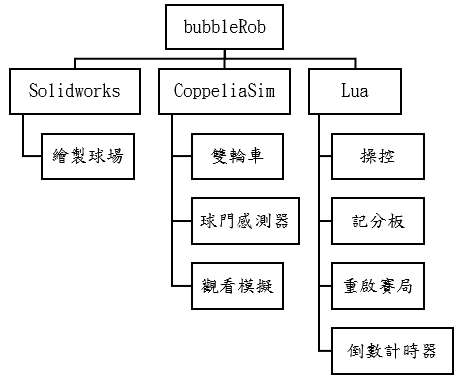
\includegraphics[width=10cm]{ag6設計架構}
\caption{\Large 設計架構圖}\label{fig.ag6設計架構}
\end{center}
\end{figure}

\section{規則說明}
類似於足球遊戲,一開始時球會置於場中央,遊戲開始後兩方即可以鍵盤操控機器人推球至已方的球門得分。\\
遊戲規則如下:
\begin{enumerate}
\item 球觸碰到情們感測器即算得分。
\item 最快獲得5分的隊伍即獲勝。
\item 任一方進球得分後,遊戲會重置,雙方回到場中央重新開球。
\end{enumerate}

\renewcommand{\baselinestretch}{0.5} %設定行距
%=---------------------參考文獻----------------------=%
\addcontentsline{toc}{chapter}{參考文獻} %新增目錄名稱
\newpage
\renewcommand\bibname{參~考~文~獻}
\begin{thebibliography}{99}  % 參考文獻印出之編號最寬為兩個字母寬
\bibitem 1\href{https://towardsdatascience.com/adam-latest-trends-in-deep-learning-optimization-6be9a291375c}{https://towardsdatascience.com/adam-latest-trends-in-deep-learning-optimization-6be9a291375c}
\bibitem 2\href{https://towardsdatascience.com/derivative-of-the-sigmoid-function-536880cf918e}{https://towardsdatascience.com/derivative-of-the-sigmoid-function-536880cf918e}
\bibitem 3\href{http://www.incompleteideas.net/book/RLbook2020.pdf}{http://www.incompleteideas.net/book/RLbook2020.pdf}
\bibitem 4\href{https://medium.com/change-the-world-with-technology/policy-gradient-181d43a24cf5}{https://medium.com/change-the-world-with-technology/policy-gradient-181d43a24cf5}
\bibitem 5\href{https://livebook.manning.com/book/grokking-deep-reinforcement-learning/chapter-11/v-11/38}{https://livebook.manning.com/book/grokking-deep-reinforcement-learning/chapter-11/v-11/38}
\bibitem 6\href{http://ukko.life.nctu.edu.tw/~u0517047/usage.html}{http://ukko.life.nctu.edu.tw/~u0517047/usage.html}
\bibitem 7\href{https://lilianweng.github.io/lil-log/2018/04/08/policy-gradient-algorithms.html}{https://lilianweng.github.io/lil-log/2018/04/08/policy-gradient-algorithms.html}\label{R.Policy Gradient}
\bibitem 8\href{https://uupgrade.medium.com/python-那些年我們一起玩過的遊戲-三-打磚塊-d89b648896ca}{https://uupgrade.medium.com/python-那些年我們一起玩過的遊戲-三-打磚塊-d89b648896ca}
\bibitem 9\href{https://cvfiasd.pixnet.net/blog/post/275774124-深度學習激勵函數介紹}{https://cvfiasd.pixnet.net/blog/post/275774124-深度學習激勵函數介紹}
\bibitem 0\href{https://www.coppeliarobotics.com/helpFiles/}{https://www.coppeliarobotics.com/helpFiles/}
\bibitem 1\href{https://hackernoon.com/the-reason-behind-moving-in-the-direction-opposite-to-the-gradient-f9566b95370b}{https://hackernoon.com/the-reason-behind-moving-in-the-direction-opposite-to-the-gradient-f9566b95370b}\label{OGD}
\bibitem 2\href{https://ruder.io/optimizing-gradient-descent/}{https://ruder.io/optimizing-gradient-descent/}
\label{OGD2}
\bibitem 3\href{https://reurl.cc/43XjEL}{https://zh.wikipedia.org/wiki/HSL和HSV色彩空間}
\label{RGBtoHSV}
\bibitem 4\href{https://reurl.cc/gzMm4N}{https://gist.github.com/karpathy/a4166c7fe253700972fcbc77e4ea32c5\# file-pg-pong-py}\label{R.pong1}
\bibitem 5\href{https://reurl.cc/95172Y}{https://github.com/schinger/pong\_ actor-critic/blob/master/pg-pong-ac.py}\label{R.pong1.1}
\bibitem 6\href{https://gist.github.com/etienne87/6803a65653975114e6c6f08bb25e1522}{https://gist.github.com/etienne87/6803a65653975114e6c6f08bb25e1522}\label{R.pong2}
%\bibitem 7\href
%\bibitem 8\href
%
%\bibitem 3\href{https://blog.csdn.net/Csdn_Darry/article/details/107142216}{https://blog.csdn.net/CsdnDarry/article/details/107142216}
\end{thebibliography}
\newpage
%=---------------附錄-----------------=%
\addcontentsline{toc}{chapter}{附錄} %新增目錄名稱
\begin{appendix}
\renewcommand{\thesection}{\bf 附錄 \Alph{section}}%設定標題名稱
\begin{center}
\fontsize{20pt}{0em}\selectfont\bf 附錄
\end{center}
\section*{LaTeX}
LaTex 為一種程式語言,支援標準庫 (Standard Libraries) 和外部程式庫 (External Libraries),不過與一般程式語言不同的是,它可以直接表述 Tex 排版結構,類似於 PHP 之於 HTML 的概念。但是直接撰寫 LaTex 仍較複雜,因此可以藉由 Markdown 這種輕量的標註式語言先行完成文章,再交由 LaTex 排版。
此專題報告採用編輯軟體為LaTeX,綜合對比Word編輯方法,LaTeX較為精準正確、更改、製作公式等,以便符合規範、製作。
 \begin{table}[htbp] %htbp代表表格浮動位置
			\centering%表格居中
			\caption{文字編輯軟體比較表}%表:標題
			\large%字體大小
			\label{tab_文字編輯軟體比較表:scale}
			\begin{tabular}{|c|c|c|c|c|c|c|}
			\hline
			\diagbox[width=5em]& 相容性 & 直觀性 & 文件排版 & 數學公式 & 微調細部\\ 
			\hline
			LaTeX 		&$\surd$&		&$\surd$&$\surd$&$\surd$\\
			\hline
			Word	 	&		&$\surd$&		&		&$\surd$\\
			\hline
			
			\end{tabular}
		\end{table}	

\begin{itemize} 
\item 特點:
\end{itemize}
\begin{enumerate}
\item 相容性:以Word為例會有版本差異,使用較高版本編輯的文件可能無法以較低的版本開啟,且不同作業系統也有些許差異;相比LaTeX可以利用不同編譯器進行編譯,且為免費軟體也可移植至可攜系統內,可以搭配Github協同編譯。
\item 文件排版:許多規範都會要求使用特定版型,使用文字編譯環境較能準確符合規定之版型,且能夠大範圍的自定義排定所需格式,並能不受之後更改而整體格式變形。
\item 數學公式呈現:LaTex可以直接利用本身多元的模組套件加入、編輯數學公式,在數學推導過程能夠快速的輸入自己需要的內容即可。
\item 細部調整:在大型論文、報告中有多項文字、圖片、表格,需要調整細部時,要在好幾頁中找尋,而LaTeX可以分段章節進行編譯,再進行合併處理大章節。
\end{enumerate}
\begin{figure}[hbt!]
\begin{center}
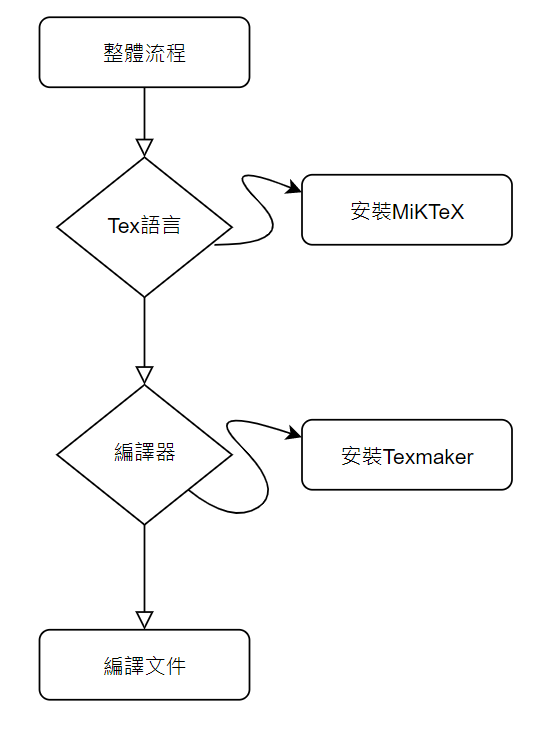
\includegraphics[width=10cm]{編譯流程}
\caption{\Large 編譯流程}
\label{fig.編譯流程}
\end{center}
\end{figure}
\end{appendix}
\section*{FFmpeg}
FFmpeg是一個開放原始碼的自由軟體,可以對音訊和視訊進行多種格式的錄影、轉檔、串流功能。在專題訓練過程中透過FFmpeg的視訊錄製的功能記錄對打影像來了解實際訓練狀況。
\newpage
\newpage
%=-------------作者簡介-----------------=%
    \addcontentsline{toc}{chapter}{作者簡介}
    \begin{center}
	\fontsize{20pt}{0em}\selectfont \bf{作者簡介}\\
	\end{center}	
	{\begin{textblock}{6}(0,0.5)
	\begin{figure}
	
\includegraphics[width=1.25in]{member1}  %作者照片
	\end{figure}
	\end{textblock}}
	{\renewcommand\baselinestretch{0.99}\selectfont %設定以下行距
	{\begin{textblock}{15}(3.5,0.7)%{寬度}(以左上角為原點之右移量,下移量)
	\noindent\fontsize{14pt}{0em}\selectfont \makebox[4em][s]{姓名}\enspace:\enspace
    \fontsize{14pt}{0em}\selectfont \makebox[4em][s]{王啟騰}\\     \hspace*{\fill} \\
    \fontsize{14pt}{0em}\selectfont \makebox[4em][s]{學號}\enspace:\enspace
    \fontsize{14pt}{0em}\selectfont \makebox[4em][s]{41023112} \\ %\makebox為文本盒子
    \hspace*{\fill} \\
    \fontsize{14pt}{0em}\selectfont \makebox[4em][s]{畢業學校}\enspace:\enspace
    \fontsize{14pt}{0em}\selectfont \makebox[9em][s]{臺北市立松山高級工農職業學校}\\
    \fontsize{14pt}{0em}\selectfont \makebox[5em][s]{\quad}\enspace\enspace
    \fontsize{14pt}{0em}\selectfont \makebox[8em][s]{機械科}\\
    \hspace*{\fill} \\
    \end{textblock}}}
   % \hspace*{\fill} \\
   \vspace{2em}
	{\begin{textblock}{6}(0,2.3)
	\begin{figure}
	
\includegraphics[width=1.15in]{member2}  %作者照片
    \end{figure}
    \end{textblock}}
    {\renewcommand\baselinestretch{0.99}
    \selectfont %設定以下行距
    {\begin{textblock}{15}(3.5,2.5) %{寬度}(以左上角為原點之右移量,下移量)
\noindent\fontsize{14pt}{0em}\selectfont \makebox[4em][s]{姓名}\enspace:\enspace
\fontsize{14pt}{0em}\selectfont \makebox[4em][s]{呂佳柔}\\ 
\hspace*{\fill} \\
\fontsize{14pt}{0em}\selectfont \makebox[4em][s]{學號}\enspace:\enspace
\noindent\fontsize{14pt}{0em}\selectfont \makebox[4em][s]{41023104} \\ 
\hspace*{\fill} \\
\fontsize{14pt}{0em}\selectfont \makebox[4em][s]{畢業學校}\enspace:\enspace
\fontsize{14pt}{0em}\selectfont \makebox[9em][s]{臺中市立臺中工業高級中等學校}\\
\fontsize{14pt}{0em}\selectfont \makebox[5em][s]{\quad}\enspace\enspace
\fontsize{14pt}{0em}\selectfont \makebox[8em][s]{機械製圖科}\\
\hspace*{\fill} \\
    \end{textblock}}}
\end{document}
